\chapter{Primeri uporabe}




\subsection{Primer uporabe modula api\_wrapper}

Enostaveno uporabo modula \verb|api_wrapper| s skriptnim delom programa Orange
prikazuje primer \ref{scripting_example}. V temu primeru pogledamo kako
u"cinkovito lahko napovemo smrtnost otrok iz raznih indikatorjev zdravja in
okolja in infrastrukture. V vrsticah $5$ do $15$ naredimo poizvedbe po
potrebnih podatkih s programskega vmesnika Svetovne banke. Nato v vrsticah $18$
do $27$ odstranimo vrstice ki nimajo ciljne vrednosti in naredimo novo tabelo z
razredom ki ga "zelimo napovedovati. Vrednosti, ki jih "zelimo napovedovati se
nahajajo v stolpcu $55$ v tabeli \verb|class_data|. Ta vrstica vsebuje podatke
o smrtnosti otrok mlaj"sih od enega leta, za leto 2015. V naslednjih vrsticah
pa zgradimo "stiri napovedne modele: naklju"cni gozd z
regresijskimi drevesi \verb|rf|, linearna regresija z regularizacijo 
\verb|ridge| in srednja vrednost \verb|mean|.
Za ocene napovednih modelov smo uporabili oceni
$RMSE$ \fnurl{https://en.wikipedia.org/wiki/Root-mean-square_deviation} in 
$R^2$ \fnurl{https://en.wikipedia.org/wiki/Coefficient_of_determination}.
Rezultate primera \ref{scripting_example} lahko vidimo v tabeli 
\ref{rezultati_skripte}.


\begin{snippet}
\begin{center}
\lstinputlisting{example.py}
\end{center}
\cprotect
\caption{Napovedovanje smrtnosti otrok do enega leta iz podatkov o dostopnosti
  "ciste vode, "stevilu bolni"skih postelj na 1000 prebivalcev in odstotku
  cepljenih otrok do drugega leta starosti.}
\label{scripting_example}
\end{snippet} 

\begin{table}
\begin{center}

\begin{tabular}{l|r|r}
  Learner & RMSE & R2      \\ \hline
 
  rf & 9.74 & 0.79 \\
  ridge & 17.76 & 0.31 \\
  mean & 21.35 & -0.00

\end{tabular}
\end{center}
\cprotect
\caption{Rezultati napovedi smrtnosti otrok do enega leta starosti.}
\label{rezultati_skripte}
\end{table} 



\section{Napoved temperature s pomočjo CO2 emisij v ZDA}


Podatke svetovne banke lahko uporabimo tudi kot "casovne vrste, z uporabo
posebnih gradnikov za delo s "casovnimi vrstami \cite{time_series}. Tukaj si
bomo ogledali enostaven primer napovedi temperature v ZDA s pomo"cjo podatkov o
emisijah. V tej napovedi smo uporabili podatke tako z gradnika WB Indicators
(Slika \ref{var_indicator_select})
kot z gradnika WB Climate (Slika \ref{var_climate_select}), 
kar prikazuje slika \ref{var_setup}. Podatke obeh gradnikov zdru"zimo v eno 
tablo Orange in s pom"cjo modela \verb|var| napovemo podatke za povpre"cno 
letno temperaturo za naslednjih nekaj let\ref{var_forecast_graph}.

\begin{figure}
\begin{center}
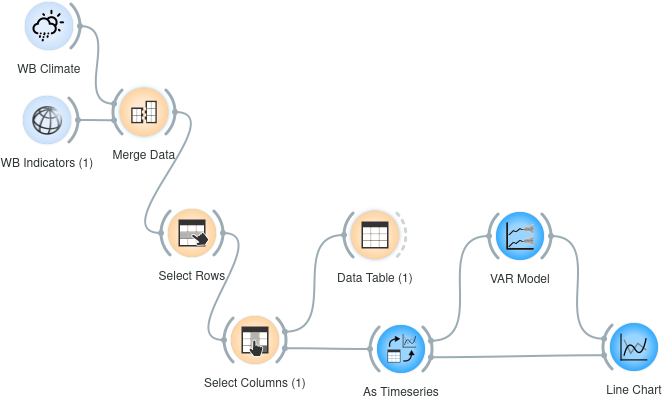
\includegraphics[width=11cm]{pic/var_setup.png}
\end{center}
\caption{Prikaz povezave gradnikov za napoved temperature.}
\label{var_setup}
\end{figure} 


\begin{figure}
\begin{center}
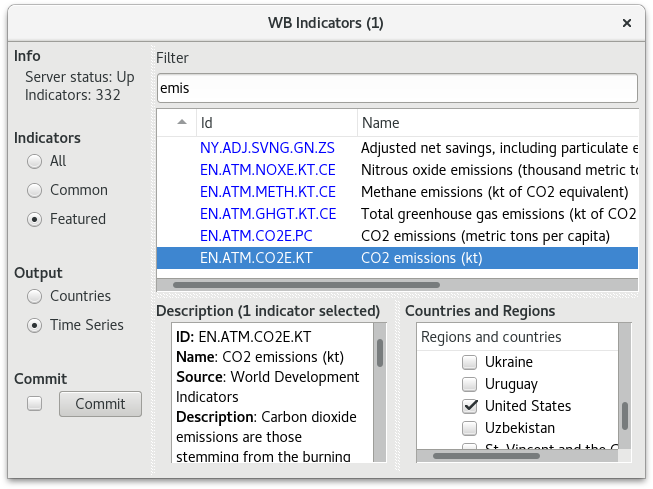
\includegraphics[width=12cm]{pic/var_indicator_select.png}
\end{center}
\caption{Izbor indikatorja CO2 emisij v ZDA.}
\label{var_indicator_select}
\end{figure} 

\begin{figure}
\begin{center}
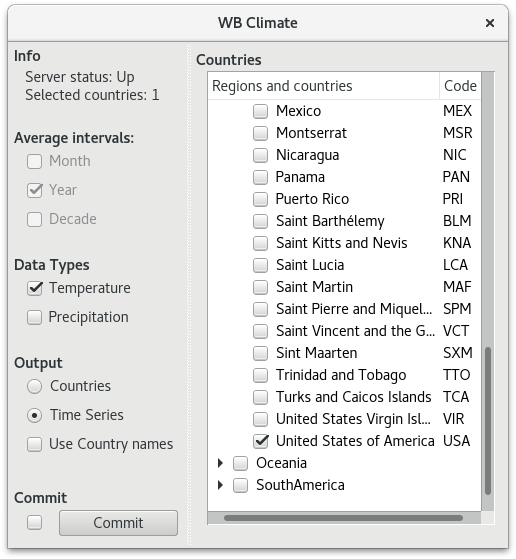
\includegraphics[width=8cm]{pic/var_climate_select.png}
\end{center}
\caption{Izbor podatkov povprečnih letnih temperatur v ZDA.}
\label{var_climate_select}
\end{figure} 

\begin{figure}
\begin{center}
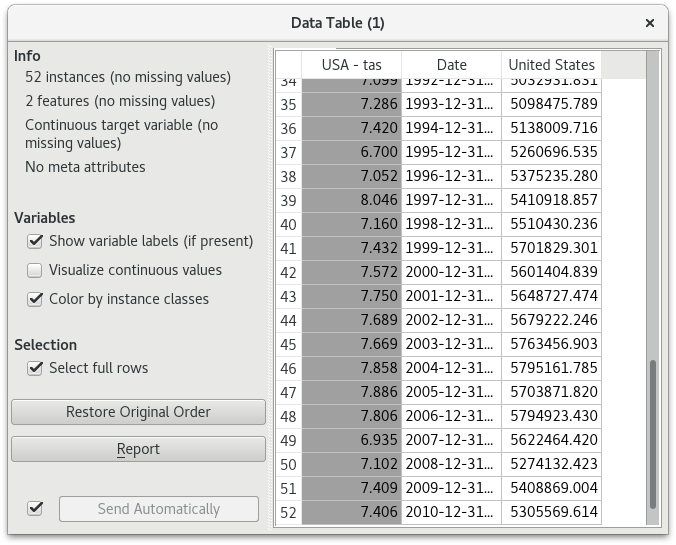
\includegraphics[width=10cm]{pic/var_data_table.png}
\end{center}
\caption{Podatkovna tabela s ciljnim razredom, in dvema poljema.}
\label{var_data_table}
\end{figure} 

\begin{figure}
\begin{center}
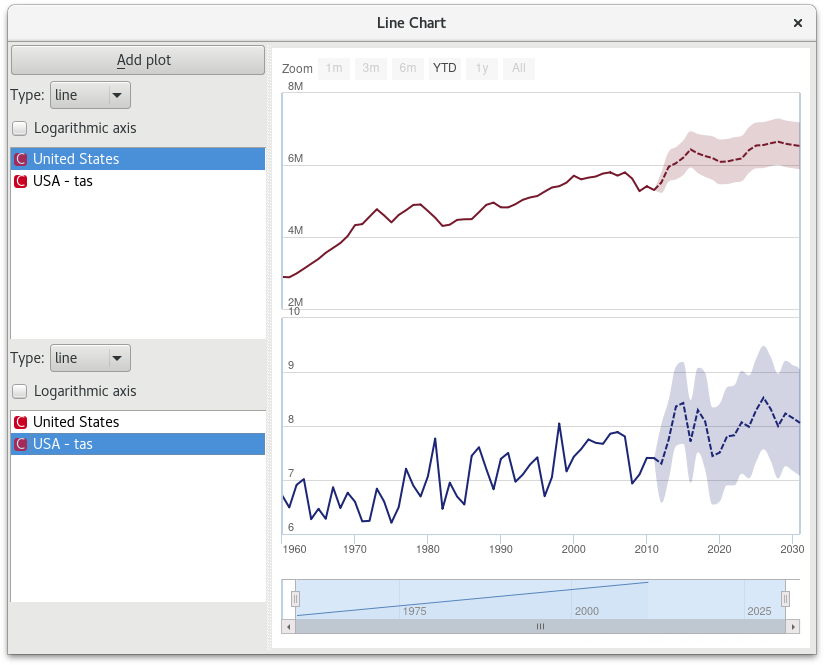
\includegraphics[width=12cm]{pic/var_forecast_graph.png}
\end{center}
\caption{Prikaz napovedi gibanja povprečnih letnih temperatur in emisij CO2.}
\label{var_forecast_graph}
\end{figure} 




\section{Clustering drzav }



\begin{figure}
\begin{center}
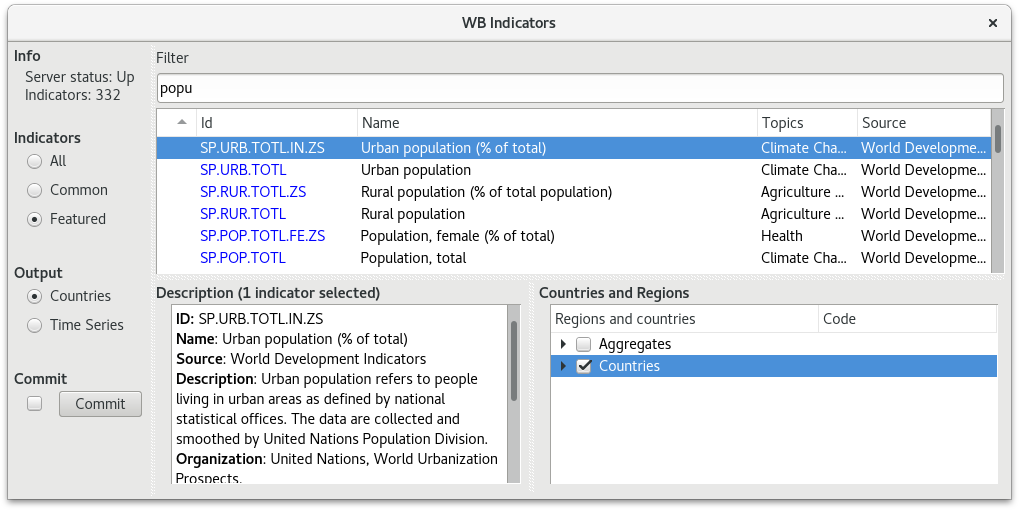
\includegraphics[width=12cm]{pic/cluster_indicators.png}
\end{center}
\caption{Izbor indikatorjev za clustering.}
\label{cluster_indicators}
\end{figure} 

\begin{figure}
\begin{center}
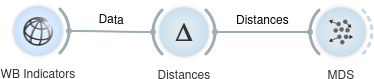
\includegraphics[width=5cm]{pic/cluster_setup.png}
\end{center}
\caption{Postavitev okalja za MDS clustering.}
\label{cluster_indicators}
\end{figure} 

\begin{figure}
\begin{center}
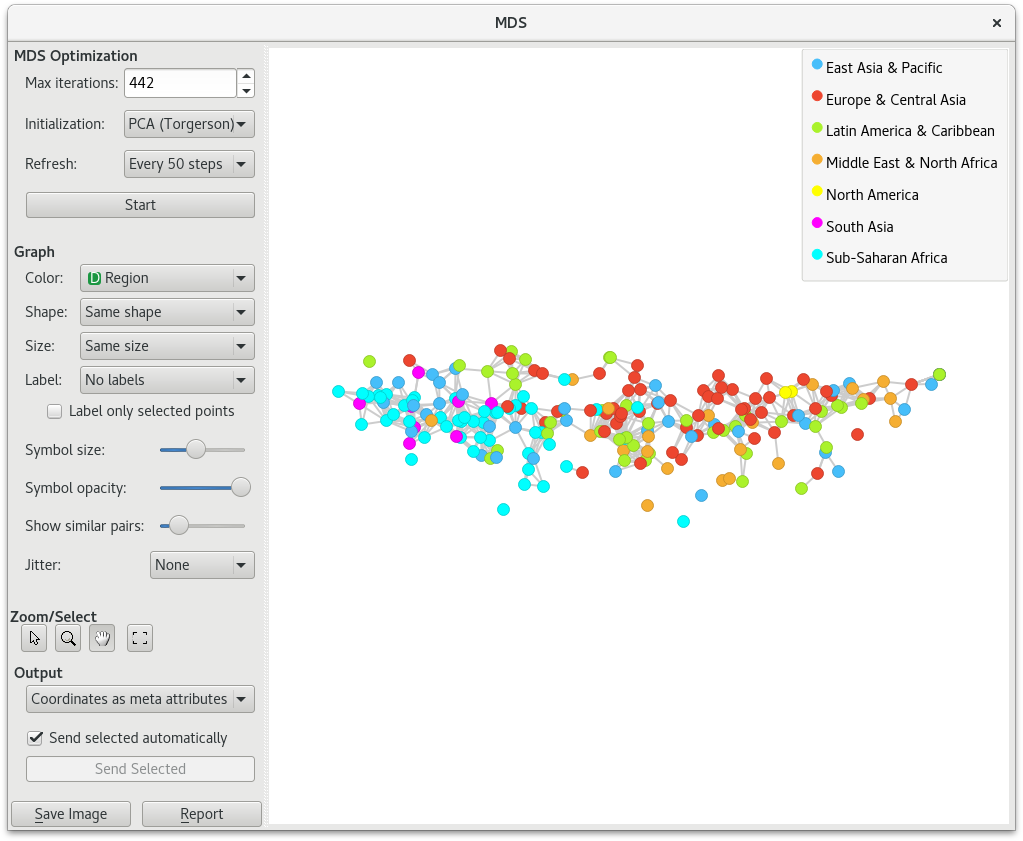
\includegraphics[width=12cm]{pic/cluster_mds_result.png}
\end{center}
\caption{Rezutat MDS clusteringa.}
\label{cluster_indicators}
\end{figure} 




